
\chapter{系统详细设计与实现}
\label{chap:achieve}

上文介绍了本系统的系统架构和涉及的技术。本章本人将进行系统各个模块的详细设计和部分的系统功能实现。

详细设计部分将通过“文档撰写与展示”、“用户空间逻辑结构”、“社交网络与门户”几个具体的功能模块,分别进行功能设计,并详细的描述每个功能的细节。

系统实现部分,由于本系统结构庞大,功能复杂,涉及许多不同体系的技术,所以限于篇幅有限,本人并不打算把系统涉及到的全部实现细节一一介绍。而只介绍其中最核心的,和最具有代表性的部分。

由于基于\smarkdown的文档撰写是本系统区别其他网络文档管理平台的最大特点。而且由于\smarkdown语法是本文作者在Markdown语法基础上扩展而来。所以介绍\smarkdown语法和它如何被渲染展示和如何被转换成\LaTeX,再进一步转换成最终的PDF文档将是本人本章介绍的重点。

由于Restful api\cite{richardson2008restful,allamaraju2010restful,fielding2000architectural,pautasso2008restful,story2009foaf}是本系统的核心架构,所以api的实现也将是本章重点介绍的内容。

\section{文档的撰写与展示}
\label{sec:writeandview}

本系统鼓励用户使用\smarkdown在系统内直接撰写文档,但是考虑到用户的使用习惯不会在段时间内改变,所以系统在用户文档的设计部分,充分考虑到了word用户可以轻松上手的功能,首先系统提供了和Word操作很相似的富文本编辑页面与\smarkdown互为补充,用户可以按照自己的喜好选择自己喜欢的编辑环境。其次系统还提供了Word等格式文档的上传与预览功能。以满足Word用户的需要。

如图~\ref{fig:xfig10}所示,用户在系统中即可以使用\smarkdown格式书写文档,也可以使用富文本方式。用户可以在编辑页面直接插入图片,系统数据库会保存用户文档数据和相应的图片文件,然后通过转换成html格式进行预览。由于本系统是用户个人文档管理功能为主的系统,所以系统默认的文档浏览权限都是私有的,也就之只用用户本人可以浏览与编辑\footnote{文档编辑和浏览权限将在社交功能小节描述}。除此以外,系统可以把保存的数据通过格式转换引擎转成\LaTeX格式的文档并可以导出。还可以进一步生成为最终的PDF文档并导出。那么就实现了,用户只关心自己的文章内容,而文章的格式则有系统预设的多种格式的模板来自动设置。常用的格式模板都以\LaTeX格式模板形式提供,用户文档和模板的组合生成都在服务器端完成,用户不用安装任何软件也不用做任何的繁琐配置。只要对\smarkdown的简单语法略有了解,就可以完成科技论文等格式要求严格的文档的写作。并直接获取到最终排版好的的PDF文档。当然,如果用户对\LaTeX格式有一定了解的话,也可以在书写\smarkdown文本的时候添加\LaTeX语法片段。这样就可以更精细的控制文档的格式。系统将陆续提供各大主流院校的毕业论文格式模板,和国内外知名出版社要求的期刊论文格式模板,以满足高校用户写论文的要求。用户只要在导出论文最终文档时 选择要导出的文档格式模板,那么就可以获取到相应格式最终文件,和文档的内容完全无关。这样也带来了另外一个好处,用户无需修改自己的文档,就可以轻松的把自己的文章转投到多家出版社。如果使用Word编辑工具是完全做不到的。\footnote{如果用户使用富文本方式书写文档那么,导出\LaTeX和使用模板生成PDF文档功能将不可用,但是对于初级用户用来编写个人博客和笔记还是非常够用的。}
\begin{figure}[H]
  \centering
  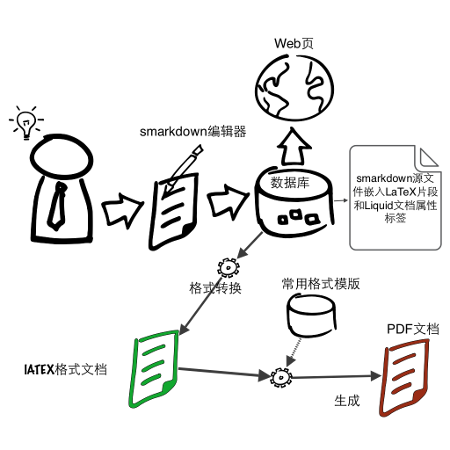
\includegraphics{writing}
  \caption{}
  \label{fig:xfig10}
\end{figure}

此外,系统在文档撰写功能部分还提供了。基本的版本控制功能,用户在建立文档时,可以定义此文档是否使用版本控制。如果使用,用户的每一次提交改变都会记录到系统,并且用户可以把文档恢复到任何一次提交以前的状态。但是每次修改文档都需要手动提交,并写明提交注释,所以建议在撰写重要的科技文档和书籍是使用。如果不使用,则系统不会保存文档的历史版本,文档的改变及时生效,定时保存。建议在笔记,博客等不重要的文档中使用。

\section{用户空间逻辑结构}
\label{sec:personstructure}

上文中曾经批评过Windows操作系统的文档管理中目录结构松散,与缺乏标签管理等问题。那么,本系统中的文档组织又是什么样的呢? 如图~\ref{fig:xfig11}所示,显然,本系统的文档组织也是由目录组成。但是这里的目录的概念和window操作系统中的目录概念不太一样。本系统的文档组织有如下特点:
\begin{enumerate}
\item 每一篇文档都隶属一个目录。
\item 每篇文档都由文档内容和若干文档属性组成,在编辑文档内容的时候,可以插入文档属性到内容中。文档显示的时候,插入的文档属性可以以用户选取的方式显示在文档中。文档有哪些属性由用户自定义\footnote{系统会预设一些常用的属性列表}。
\item 隶属于一个目录中的文档具有相同的属性,该属性列表由目录属性设定。每个目录需要定义一个属性列表。并定义属性的必要选项,比如必填,选填等。
\item 每个目录还必须设定一个文档默认显示方式,对于只有属性没有内容的文档。将使用目录中定义的默认模板显示属性。
\item 每个目录可以设定一个目录的首页模板,也就是用户访问该目录文档列表的时候显示的页面。系统将预设一些常用的页面,用户也可以自己定义。
\item 如果每个目录都从头自定义属性,那么使用起来会非常不方便。所以系统提供了目录继承功能。也就是新建目录的时候可以选择一个已有的目录继承,继承的内容包括属性列表、默认内容模板,目录首页模板等。目录继承可以使用强制和非强制的方式,强制继承方式要求子目录不可以删除父目录定义的属性,但是可以增加自己的属性。非强制继承不要求子目录一定设置父目录属性,只在建立时复制了父目录的属性。\footnote{目录继承不限于个人空间内,也可以通过目录继承共享继承其他用户的目录结构后面的章节将介绍。}
\end{enumerate}

不难看出,比起相对松散的windows系统的文件管理,文档在本系统中的组织形式更加严密,结构也更加复杂。如此设计的目的在于借助系统级的某些强制约定来帮助用户形成规范的文档管理习惯。每个目录中的文档必须有相同的属性在某种程度上强制用户把某一类内容很相近的文档放到同一个目录中。而文档中可以插入属性的功能,保证了文档内容的灵活性与规范性的平衡。而目录的继承功能则保证了系统即可以被配置成功能复杂的信息管理系统,也可以通过非常简单的方式提供给刚刚使用系统的用户使用。以上描述获取不能清楚的表达设计用意,下面举几个简单的例子:
\begin{itemize}
\item 假如目录A如此设置:文档属性只保留一个“任意文件类型”属性,目录的首页模板使用资源管理器模板,文档默认显示模板为显示文件内容。文档内容页留空。那么目录A就变成了一个网络磁盘应用。
\item 假如目录B如此设置:文档属性只保留一个“图片文件类型”属性,目录的首页模板使用图片幻灯片模板,文档默认显示模板为显示图片内容,文档内容页留空。那么目录B就变成了一个云端相册应用。
\item 假如目录C如此设置:文档属性设置为空,目录的首页模板使用文档摘要列表,文档默认显示模板为空。文档内容页我们可以写我们的文章,那么目录C就变成了一个网络日志应用。
\end{itemize}
综上所述,本系统即可以为初级用户提供简单的,易于使用的常用功能,这些功能不需要用户对系统有任何了解也可以无障碍的使用。又可以为高级用户提供十分复杂而强大的,具有极强的可配置性的高级功能。熟练使用本系统的用户可以使用本系统段时间内完成一个功能复杂的数据管理系统。

有一些编程经验的读者通过以上的描述可能已经发现了,本系统的目录和文档的结构设计与面向对象的编程的思想及其类似。系统中的目录就相当于面向对象系统中的类,而文档就相当于面向对象系统中的对象。属性就相当于面向对象系统中的属性。唯一缺少的是对象方法。由于本系统为文档管理系统。所以之需要文档为我们保存信息,而不需要做什么其他的事情,所以自然并不需要额外的方法。当然如果读者愿意,把文档的内容,目录的首页模板等理解为对象方法和类方法也完全可以。

以上多次提到文档属性,那么到底可以定义那些种文档属性呢?下面简单说明一下系统提供哪些类型的文档属性:
\begin{itemize}
\item 整数
\item 浮点数
\item 布尔值
\item 枚举值
\item 级联枚举值
\item 短字符串,纯文本
\item 大段字符串,纯文本
\item 大段字符串,富文本(\smarkdown)
\item 任意类型文件
\item 制定类型文件(Word,PDF,EXCEL等)
\item 图片
\item 视频
\item 链接
\item 表格数据
\item 日期时间
\item 数学公式,化学式,电路图等特殊专业的编辑器属性(\LaTeX格式)
\end{itemize}
除此意外还有一些高级的系统属性:
\begin{itemize}
\item 认证属性。此属性的功能将在后面小节详细介绍。
\item 由其他属性计算出结果的编程字段。\footnote{此功能计划使用R语言作为扩展语言,由于功能复杂度可能较高并不在目前版本中实现}
\end{itemize}
系统属性类型将随着系统的更加深入的使用,逐渐积累完善。以实现完整的系统生态环境。
\begin{figure}[H]
  \centering
  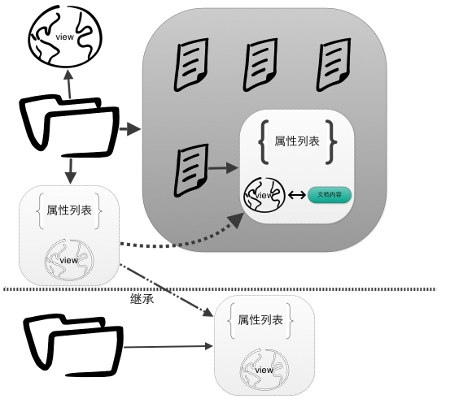
\includegraphics{person_s}
  \caption{用户空间逻辑结构}
  \label{fig:xfig11}
\end{figure}

当然,为来让用户更快上手使用系统,系统不会给用户直接提供一个“空壳”让用户自己建立目录结构。系统预设会给每个用户提供一个初始的目录结构。一方面,用户可以很快上手使用系统的常用功能,而无需花时间去了解系统中复杂的配置。另外一个方面,系统提供的预设的目录也是高级用户日常使用系统最常使用的部分。系统预设的目录包括:
\begin{description}
\item[我的简历] 存放用户的个人简历,由特定组织用户进行认证。
\item[我的成果] 主要保存用户完成的学术成果,包括发表的期刊论文,会议论文等。此目录结构继承自图书馆的一个共享目录,用户插入到此目录的文档可以申请图书馆的文献信息补全,和文献认证服务。
\item[我的著作] 主要保存用户编著的书籍。
\item[我的毕业论文] 针对学生用户,存放他们的毕业论文。此目录结构也继承自图书馆的一个共享目录,用户插入到此目录中的文档可以申请毕业论文提交服务。
\item[我的笔记] 可以添加用户笔记,此目录中的文章默认访问权限为私有。
\item[我的博客] 可以添加用户博客,此目录中的文章默认访问权限为公开。
\item[我的参考文献] 保存用户的参考文献,此目录也继承自图书馆的一个共享目录,图书馆提供参考文献信息服务。用户可以直接从图书馆目录中获取参考文献信息,并且可以导出多种格式,在用户使用\smarkdown撰写文章的时候,可以直接从该目录下选取文献,进行添加。省去了调整参考文献格式的时间。
\item[撰写中论文] 在该目录下,用户可以编写自己的科技论文,也可以通过继承该目录来自己定义章节书写论文。
\end{description}
以上为系统预设的一些目录,由于有些目录为学院业务必须。所以预设目录用户无权删除。用户也可以自己定义目录,以及通过继承预设目录来完成更多个性化配置。

另外,前文一直提到的标签体系也在本系统中得以实现,系统中的每一篇文档都可以被用户定义某些标签,这些标签既可以通过系统提供的预设列表中选取,也可以由用户自己定义。有了标签系统的帮助,用户可以很方便的查找自己的文档。不过标签系统,在本系统不叫“标签”这个名字,而是叫做“主题(Topic)”,系统将根据标准的专业和研究领域预设一个主题树供用户使用。关于主题将在下一节继续讨论。

\section{社交网络与门户}
\label{sec:society}

作为一个网络时代的信息系统,如果没有社交网络功能是怎么也说不过去的。所以社交网络也是本系统的一个功能特点,也是本系统区别于其他校园信息系统的一个重要特色。如上文所述,使用本系统,用户可以方便的在自己的多个设备中共享个人文档,并可以利用系统方便的撰写科技文献。但是,用户有时并不满足于孤立的保存文档。有时,用户希望可以把自己的文档方便的分发给自己的学生或者工作伙伴,也有的时候用户可能希望自己的某些文档可以在网络上被任何人访问到,可以被搜索引擎搜索到。设置有的时候用户可能希望和自己的项目组成员一起合作完成文档。要实现这些功能就需要系统拥有完备的社交网络和门户功能。下面就分别就“组织结构和用户认证”、“主题与分类”、“好友与关注”、“系统门户”、“个人门户与评论”、“用户组与用户群”、“目录共享和信息服务”、“用户邀请和提及系统”等几个方面分别介绍系统的社交网络功能。

\subsection{组织结构和用户认证}
\label{sec:auth}

本系统面对的用户为高校的教师和学生,所以系统用户信息需要包括用户的所属的学校、学院和专业等信息。也就是说系统用户基本上是以实名制登录系统。系统提供用户认证功能来确保用户个人信息的真是性。所以,系统管理中不需要为用户发文的信息审查问题担心\footnote{中国的信息审查制度确实是开放系统的天敌,实名制的系统要承担的责任要小很多。}。为用户搭建组织结构带来的另外一个好处是,在系统公共首页(总门户)中可以根据用户所在的学院专业快速导航到用户的个人空间和直接浏览某学院或专业中所有公开的文档。

用户认证机制,本系统将使用用户自己注册并由特定组织用户进行认证的方式和OAUTH认证协议\footnote{一种流行的获取统一用户信息的协议,通过该协议用户可以通过安全的方式获取到其他公共系统的用户信息,比如现在很多网站上的以qq,或者微博身份登陆的功能就是使用该协议。}的方式相结合。组织结构将分成三级 学校,学院,和专业,所以用户注册的时候只需填写用户名,密码,姓名,唯一标示(教师的工资号,学生的学号)和所属的单位信息即可。其余用户信息,比如性别,年龄等都被定义在用户的简历文档目录中的文档中。简历文档目录是一个预设目录,限制只能建一篇文档,该文档保存用户个人信息,并存在认证字段。

\subsection{主题与分类}
\label{sec:topic}

本系统的每一个文档都可以被标示上若干标签,标签的作用是标示此篇文档与哪些主题相关。标签可以由用户自己填写,填写的过程中系统会根据系统已有的标签进行提示。如果系统中已经有了相同的主题,用户可以直接选择。

系统建立只初,按照标准的学科与研究领域,预设了大量与各专业相关的主题。主题系统可以帮助用户快速的检索到自己的文档,也可以帮助系统浏览者快速的浏览到自己感兴趣的主题文档和导航到相关专家的个人空间。

为了减少用户为文档录入主题的操作。系统的目录可以设定默认主题,目录下的所有文档会自动填写上目录所设定的主题。

\subsection{好友与关注}
\label{sec:friend}

添加好友是一个社交系统的必备功能,近年来,随着微博等系统的流行,关注其他用户也成为了很多系统流行的功能,如果某用户follow了某个其他用户,那么该用户发布的任何有权限浏览的文档都会自动的推到该用户的管理首页上。比如,github就具有这样的功能。

所以本系统将同时支持添加好友,和follow用户功能。添加后的用户将放入用户的通讯录中。在用户撰写文档,分发文档的时候可以直接从通讯录中选取。follow后的用户文档,将自动发布在管理界面的首页。但是,本系统毕竟是一个文档管理系统,而非以社交交流为主的系统,所以目前系统并不提供微博系统中常用的转发,评论转发等功能。用户交流可以通过文档评论功能,和私信功能完成。

\subsection{系统门户}
\label{sec:global}

本系统结构设计采用分布式建库模式,为每一个用户(老师与学生)建立自己的存储空间,用户可以自己管理自己的空间,并提交(上传)数据。除此以外,系统为用户提供了三个可以浏览用户文档的系统门户,分别是个人门户,组门户和总门户,三个门户的关系如图~\ref{fig:xfig12}所示。
\begin{description}
\item[总门户] 即系统统一的发布页面,也是系统首页显示的内容,任何访问者通过该页面可以进行统一的浏览与检索。搜索引擎爬虫也可以搜罗本页面中的信息。页面中显示最新发布的用户文档,和按照组织结构和主题进行分类导航的功能。访问者点开用户文档的时候即被导航到该用户的个人空间中该文档的显示页。
\item[个人门户] 即用户的个人空间,可以显示用户设定为公开的任何文档。用户可以自定义该页面的模版。
\item[组门户] 即用户组的空间,组中任何用户都可以把文档公开到该空间,关于用户组,将在下面小节讨论。
\end{description}

用户可以自由的设定文档的公开范围:
\begin{itemize}
\item 设定为私有的文档只能在自己的管理界面获取,三个门户都不显示,而且搜索引擎也无法获取,以保证文档的绝对安全。
\item 用户可以选择是否发布到个人门户,或者某个用户组门户,用户可以多选。发布到组门户的文档可以选择组私有或者组公开。
\item 已经被发布到个人门户的文档可以选择是否公开到总门户,被公开的文档可以被总门户检索和导航到。
\end{itemize}

\begin{figure}[H]
  \centering
  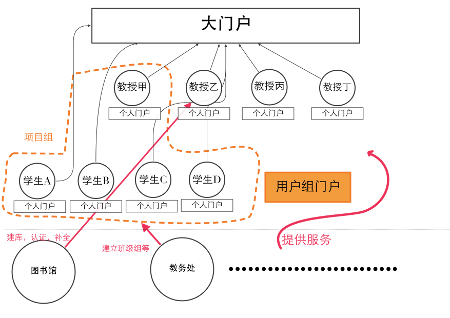
\includegraphics{global}
  \caption{三个系统门户}
  \label{fig:xfig12}
\end{figure}

\subsection{用户组与用户群}
\label{sec:team}

系统支持两中类型的用户组:team和group,即用户组和用户群。

用户组比较类似qq中的群,由一个某一用户建立,可以通过管理员添加或者用户申请方式添加组成员。建立者可以制定某几位用户为组管理员,管理员有权利添加和删除组成员和对组门户进行维护。包括开启和关闭组门户,为组门户更换主题等操作。也可以控制那写组成员可以发布哪些类型的文档。组门户是用户组公开组内文档的地方,用户发布到用户组的文档可以选择发布成共有或者私有,私有文档只有组内用户进入管理界面后通过登陆组空间才可以访问。共有文档则直接发布到组门户。实际应用中,用户组被设计用来定义项目组、班级等长期需要共享文档和交流的组织。

用户群的功能较少,它只是对用户联系人的一个简单分组,为了设定共享目录或者群发消息时更便捷。

\subsection{用户邀请和提及系统}
\label{sec:ins}

社交系统的一个很大的特点是使用的用户群越大,系统的易用性越强,系统的作用也就越明显。比如某老师的同事和学生都不是本系统的用户,那么本系统对于该老师来讲就是一个单纯的个人文档管理系统,而想要分发和共享自己的文档给别人依然很麻烦。如果他周围的人都是本系统用户,那么社交网络的便捷就发挥出来了。所以本系统提供了一个用户邀请功能,用户如果想要使用本系统共享某些文档给不是本系统用户的人,这时他可以通过本系统提供的邀请功能,给他发一封电子邮件,或者短信。那个人收到信件后,只要登陆系统就可以成为系统用户,并自动成为该用户的好友。这样的功能不仅方便了用户分发文档,而且也有助于系统快速建立社交网络。

还有一种情况是某用户和一个项目组里的一些人一起写了一篇文献,在填写文献作者的属性里该用户填写了其他成员的姓名拼音或者名字。那么,和该拼音或者姓名相同的用户在登陆的时候,系统就会提示,有一篇文献需要认领。如果本人确认其是该文献的作者之一,那么这篇文献将自动被复制进该用户的空间。同时该文献的作者姓名列表相应的名字会被点亮,可以直接链接到用户的个人门户。

另外一个功能,本系统借鉴了微博平台,即“提及”功能。如果用户在文档或者评论中使用了“@+用户名”的方式。则被提及的用户将在登陆系统时在提及一栏中收到消息。

\subsection{目录共享和信息服务}
\label{sec:informationservice}

除了以上社交平台普遍支持的功能以外,本系统还支持一个其他社交平台并不支持的功能,目录与文档共享功能与文档的认证服务功能。下面分别对这两部分功能进行设计。

\subsubsection{目录共享}
\label{sec:foldshare}

如前文所述,系统目录可以继承本用户其他目录,以获取相同的属性和默认模板等信息。除此之外,系统还支持继承其他用户的目录,前提条件是该目录被用户设定为共享。目录共享具有两层含义:
\begin{enumerate}
\item 目录信息可以被其他用户继承。
\item 目录对其他用户开启推送文档权限(post服务)。
\end{enumerate}
系统并不支持用户直接向其他用户目录直接添加文档,所以需要先继承共享的目录,然后在自己的空间中编辑好文档,并推送到其他用户的共享目录。用户在共享目录时,可以选定共享的范围,也可以选定用户可以推送的文档数量,甚至可以关闭推送,只允许继承目录。

如图~\ref{fig:xfig13}所示,目录共享功能不仅支持简单继承与推送功能,它还支持反向推送等高级特性,一下是目录共享特性的一些原则:
\begin{figure}[H]
  \centering
  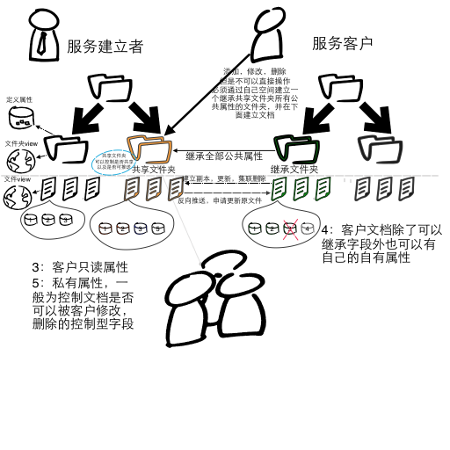
\includegraphics{share}
  \caption{目录共享}
  \label{fig:xfig13}
\end{figure}
\begin{enumerate}
\item 任何用户都在自己的空间中编辑,要想给别人编辑也是继承了共享,然后推送文件到他人空间。
\item 服务提供者,有对共享文件夹中文件的绝对控制权。
\item 共享文件夹可以控制是否还可以继续共享,或者可以推送文章。
\item 共享属性分为公有,私有,保护,私有的客户无法看到,保护的用户可以看到但是无法修改。
\item 共享文件夹中的文件view以本用户文件夹为准。
\item 系统属性中有特殊的系统类型,以控制文档是否可以被客户推送修改和集联删除。
\item 反向推送,可以更新推送源文件,但是需要客户确认,客户可以设定自动确认,推送时选定。
\item 文件夹继承属性,可以寻找用户,就可以看到其下的共享文件夹,不共享的文件夹不可见,但是未必起初选定继承的文件夹可以推送,公有和保护属性齐全,属性名和类型一致即可推送。
\item 一个文件夹内的文档属性固定,必须由文件夹确定,但是view可以自己定义,当然缺省使用文件夹定义的文档view。
\item 认证类型属性,可以绑定一个或者多个字段,绑定的字段如果有变化,认证信息及变回未认证状态。
\end{enumerate}

如上所述,所以目录共享不仅是信息共享的高级使用方式,也是是文档认证等信息服务的基础。当然共享目录功能使用相对复杂,对于日常使用本系统作为文档管理功能的用户很少会用到。但是如果用来搭建信息服务,目录共享确实可以派上用场。

\subsubsection{信息服务}
\label{sec:service}

目录共享的一个常用场合就是用来搭建信息服务,如果一个用户想要收集一些信息,就可以把一个设置好字段目录共享,然后其他用户就可以通过共享该目录向该目录中推送文档,而且文档的字段都一样的,就像一个小型的数据库。这样一个信息的收集过程本身就是一个信息服务平台。而且系统的任何用户都可以成为服务的提供者,也可以是服务的客户。

系统最具有特点的信息服务即文档认证服务。认证服务的设计灵感来自于微博系统的用户认证,本系统对其进行来扩充,即系统中任何用户都可以认证其他用户的文档。当然,认证者需要具有一定权威性,经过他认证的文档才有一定的可信度。比如,用户默认目录“我的成果”就继承自图书馆的一个具有认证字段的目录。因为图书馆这个用户可以通过检索各大数据库来确认用户的成果是否已经发表在某些刊物上,它具有一定权威性。所以经过图书馆认证的成果,被任何人浏览的时候都具有很高的可信度,甚至学校进行业绩考核时,也可以对这些认证信息进行参考。

认证的流程是这样的,认证提供者先共享一个具有认证字段的目录,其他用户继承该目录,并推送文档到该目录,认证提供者看到推送的文档如果满足要求,则对其进行认证,然后反向推送回去,那么客户的用户空间中的文档就具有来认证信息。该文档在门户中显示的时候会带着认证的信息。认证字段可以和多个字段进行绑定,如果这些字段进行来修改。那么认证信息将自动消失,这时用户需要重新认证。

通过以上描述,我们看到通过目录共享带来的灵活配置。用户可以以本系统为基础构建很多有趣的信息服务,甚至搭建属于自己的小型信息管理平台。更多信息服务的构建方法,可以留给用户自己去探索发现。

\section{\smarkdown语法}
\label{sec:smarkdownsyntax}

\smarkdown是以markdown语法为基础,并增加了学术文档中常用的表格、脚注、参考文献、代码块、属性列表、目录等语法内容,并且可以添加\LaTeX语法片段和文章属性字段。文章属性字段通过Liquid模板语言嵌入到文档中,并通过预处理机制替换成实际的内容。然后把替换后的文本交由\smarkdown引擎处理成xhtml格式进行显示。下面就分markdown基础语法、smarkdown扩展语法、嵌入属性语法、嵌入\LaTeX语法几个部分分别进行介绍。

\subsection{markdown基础语法研究}
\label{sec:markdownbase}

\begin{description}
\item[段落] 一个段落是由一个以上的连接的行句组成,而一个以上的空行则会划分出不同的段落(空行的定义是显示上看起来像是空行,就被视为空行,例如有一行只有空白和 tab,那该行也会被视为空行),一般的段落不需要用空白或换行缩进。
\item[标题] Markdown 支持两种标题的语法,Setext 和 atx 形式。Setext 形式是用底线的形式,利用 = (最高阶标题)和 - (第二阶标题),Atx 形式在行首插入 1 到 6 个 \# ,对应到标题 1 到 6 阶。
\item[区块代码] 区块引用使用 email 形式的 '>' 角括号。
\item[强调] Markdown 使用星号和底线来标记需要强调的区段。比如:*强调*、\_强调\_、**强调** 都表示加粗显示。
\item[无序列表] 无序列表使用星号、加号和减号来做为列表的项目标记,这些符号是都可以使用。
\item[有序列表] 有序的列表则是使用一般的数字接着一个英文句点作为项目标记。
\item[链接] Markdown 支援两种形式的链接语法: 行内 和 参考 两种形式,两种都是使用角括号来把文字转成连结。行内形式是直接在后面用括号直接接上链接,参考形式的链接让你可以为链接定一个名称,之后你可以在文件的其他地方定义该链接的内容。
\item[图片] 图片的语法和链接很像,只不过把链接的地址换成图片的地址。本系统中,用户要向文档添加图片非常方便,可以直接填写网络图片库的图片地址,也可以从本机上传图片,上传后系统将自动为用户填写好Markdown的图片语法。
\item[嵌入HTML] 在一般的段落文字中,你可以使用反引号 ` 来标记代码区段,区段内的 \&、< 和 > 都会被自动的转换成 HTML 实体,这项特性让你可以很容易的在代码区段内插入 HTML 码。
\end{description}
虽然Markdown语法简单易学,而且在网络时代非常流行,被越来越多的网络编辑系统所采用,但是它只定义了网络媒体中常用的表达方式,用来书写科技文档还略显不足。所以本系统在Markdown基础语法的基础上对其进行了扩展,以满足书写科技文档常用的格式需求。

\subsection{\smarkdown扩展语法}
\label{sec:smarkdownextr}

\begin{description}
\item[表格] 如下例子所示,表格第一行包含列标题,第二行包含位于标题和内容之间的强制性分隔线,接下来的每一行就是表格的内容。列与列之间用竖线 | 分隔。如果愿意的话,可以在表格每一行的开头和结尾处添加竖线 |。输出的结果一样。通过在对应列的分隔线添加冒号 : 可以指定列的对齐方式。冒号 : 在分隔线的左边说明此列左对齐,冒号 : 在分隔线的右边说明此列右对齐,冒号 : 在分隔线的左右两边说明此列居中。
  \begin{bframe}
    Col1     |                  标题                   |               标题                  |\\
    - - - - -|:- - - - - - - - - - - - - - - - - - - :|- - - - - - - - - - - - - - - - - -:|\\
    cell     |                中间对齐                 |              右对齐                 |\\
  \end{bframe}
\item[脚注] 脚注是在需要标记脚注文字的后面增加一个方括号,方括号中的内容必须以  \^{} 开头,再接着是数字、字符串标记,接着,在文件的任意地方,你可以把这个脚注的内容定义出来.例如:
  \begin{bframe}
    Footnotes[\^{} 1] have a label[ \^{}label] and a definition[\^{}!DEF]\\
    %[\^{} 1] This is a footnote
    %[\^{}label]: A footnote on "label"\\
    %[\^{}!DEF]: The definition of a footnote.\\
  \end{bframe}
\item[高亮代码块] 使用反引号,加语言名。支持多种语言,比如 python, c, html 等,。
  \begin{bframe}
    ```python\\
   def hello():\\
    return 'Hello World'\\
    ```\\
  \end{bframe}
\item[属性列表] 定义 HTML 元素的属性。可以自定义文本内容的id和css类。
\item[目录] 在需要目录出现的地方放置一个标记,这样会自动生成一个嵌套的包含所有标题的列表。默认的标记是 [TOC]。目录跳转的标题 id 是依据标题内容自动生成的,只包含英文、数字、下划线 \_ 等。对于全部是中文的标题,自动生成的标题 id 为空,导致无法跳转。可以使用属性列表方法,定义标题 id。
\end{description}
\subsection{嵌入属性语法}
\label{sec:addattr}

前文提到,任何一个文档都可以定义若干属性,在文档中可以添加这些属性。由于属性有多种类型,每种类型的表现形式也不近相同。所以系统为每一种属性都提供了若干表现方式可以供文档显示,比如:一个数字属性叫做aint,那么如果要显示该数字,并只保留两位小数,可以使用数字类型的format样式函数输出。每种类型的属性支持的样式函数不同,比如,一个pdf类型的文档就支持pagenum(页数)函数,和cutpage(取前多少页)函数。

属性插入文档的语法按照Liquid模板引擎语言设计,插入时直接用\{\{属性名.样式函数\}\}这样的结构加入到文档中,文档在被翻译成其他格式前,先进行预处理,把属性替换成显示的样子和文档一起显示。

\subsection{\LaTeX片段语法}
\label{sec:latexpic}

对于一般的科技文档撰写,系统提供的\smarkdown语法已经基本上可以满足大部分用户的需求了。但是为了满足有些数学和力学专业的用户,本系统还提供了在\smarkdown文档中直接添加\LaTeX数学公式片段的功能\footnote{由于\LaTeX片段只有在把文档转换成\LaTeX文档的时候才会编译,所以文档包含的\LaTeX片段在预览和WEB显示时无法显示完整的输出格式。}。

\LaTeX数学片段的语法很简单,直接把行内\LaTeX数学公式源代码写到文档中以\$为标志的区间内就可以。区间内的公式片段将保留到\LaTeX编译阶段直接输出公式。而将独立公式放入以\$\$.....\$\$或者[.....]的区块中就可以。

\section{RESTful api}
\label{sec:apitable}

本系统的核心架构就是一个RESTful的web service。通过这个标准的api,任何系统都可以调用本系统中用户数据和文档数据。同时它也是所有本地客户端程序访问系统的标准接口。关于RESTful api是什么,有什么样的好处,有多么流行,在前文中已经介绍过了。所以本节就直接进入主题,通过通过统一资源地址、返回内容、认证、状态码四个方面介绍本系统的api。
\subsection{统一资源地址}
\label{sec:researchurl}
RESTful规定对系统的操作有两个部分表达,资源的地址和对该地址执行的操作。地址为一个标准的URL。而操作则用HTTP协议中标准的几个动词来表达 新建、获取、修改、删除等操作,下面列出系统对于不同的操作将采取什么样的行为。
\begin{itemize}
\item \fbox{GET} 获取一个或者一些资源,系统将返回\fbox{200 ok}请求的数据。
\item \fbox{POST} 添加资源,系统将在成功添加资源后返回\fbox{201 Created}并且返回被添加的资源的数据。
\item \fbox{PUT} 修改指定的资源,系统将在成功修改资源后返回\fbox{200 ok}并且返回被修改的资源的数据。
\item \fbox{DELETE} 删除制定的资源,本系统对于删除操作采用的幂等\footnote{简单的说,就是无论对同样的资源操作多少次,结果都一样}的。也就是说无论要删除的资源是否存在,系统都返回\fbox{200 ok},表示删除成功。
\end{itemize}


上面简单描述了对资源所做操作的类型,下面将用表格~\ref{tab:api}描述一下本系统实现的RESTful api中有那些资源,这些资源获取和操作的方式是什么样的,以及可选的参数和备注。

\begin{table}[H]
  \centering
  \begin{tabular}{|c|c|c|c|}\hline
    URL & 命令  & 对URL进行的动作 & 备注\\\hline
    \char92 users & GET & 获取用户列表 & page和per\_page \\\hline
    \char92 users\char92 :id & GET & 获取指定用户 &  id为用户的id号 \\\hline
    \char92 user & GET & 获取当前用户 &   \\\hline
    \char92 users & POST & 添加用户 & 所有用户表所需字段 \\\hline
    \char92 users\char92 :id & PUT & 修改指定用户信息 & 只有管理员可以使用 \\\hline
    \char92 users\char92 :id & DELETE & 删除指定用户 &  只有管理员可以使用 \\\hline
    \char92 user & PUT & 修改当前用户信息 & 用户表所需字段  \\\hline
    \char92 user & DELETE & 删除用户 &  \\\hline
    \char92 session & POST & 登录 & 用户名、密码\\\hline
    \char92 folders & GET & 获取当前用户目录列表 & page和per\_page  \\\hline
    \char92 folders\char92 :id & GET & 查看目录页面 & id为id号或目录名 \\\hline
    \char92 folders & POST & 添加目录 & page和per\_page\\\hline
    \char92 folders\char92 :id & PUT & 修改目录页面 &  id为id号或目录名 \\\hline
    \char92 folders\char92 :id & DELETE & 删除目录 & id为id号或目录名 \\\hline
    \char92 folders\char92 :id\char92 documents & GET & 查看当前目录文档列表 & page和per\_page \\\hline
    \char92 folders\char92 :id\char92 attributes & GET & 获取目录属性列表 &  \\\hline
    \char92 folders\char92 :id\char92 attributes & PUT & 编辑目录属性列表 &  \\\hline
    \char92 folders\char92 :id\char92 documents & POST & 添加文档 & 必要字段 \\\hline
    \char92 folders\char92 :id\char92 documents\char92 :d\_id & GET & 查看文档 & d\_id为id或文档名 \\\hline
    \char92 folders\char92 :id\char92 documents\char92 :d\_id & PUT  & 编辑文档 & d\_id为id或文档名 \\\hline
    \char92 folders\char92 :id\char92 documents\char92 :d\_id & DELETE  & 删除文档 & d\_id为id或文档名 \\\hline
    \char92 folders\char92 :id\char92 documents\char92 :d\_id\char92 attributes & GET & 查看文档属性列表 & \\\hline
    \char92 folders\char92 :id\char92 documents\char92 :d\_id\char92 attributes & PUT  & 编辑文档属性列表 &  \\\hline
  \end{tabular}
  \caption{系统api}
  \label{tab:api}
\end{table}
以上表格内容为本系统最基本api资源,完成的资源列表,将在本系统发布后,由api文档给出。
\subsection{返回的内容}
\label{sec:content}

对于以上URL系统支持多种格式的返回内容,可以返回atom,xml,json等格式,由于篇幅原因这里就不一一展示各种格式的返回内容了。下面以一个用户信息的json返回结果为例说明:
\begin{bframe}

[\\
    \{\\
        ``id``: 1,\\
        "username": "steve\_ma",\\
        "email": "steve2008.ma@gmail.com",\\
        "name": "马胜",\\
        "ident\_no": "040191",\\
        "department": "图书馆",\\
        "major": "计算机",\\
        "blocked": false,\\
        "created\_at": "2012-05-23T08:00:58Z",\\
        "qq": "",\\
        "weibo": "",\\
        "dark\_scheme": false,\\
        "pingyin": "masheng",\\
        "provider": "p",\\
        "theme\_id": 1\\
       \},\\
       \{\\
        ``id``: 2,\\
        "username": "xulinyin",\\
        "email": "xuly@tju.edu.cn",\\
        "name": "许林英",\\
        "ident\_no": "0000000",\\
        "department": "计算机学院",\\
        "major": "计算机",\\
        "blocked": false,\\
        "created\_at": "2012-05-23T08:00:58Z",\\
        "qq": "",\\
        "weibo": "",\\
        "dark\_scheme": false,\\
        "pingyin": "xu lin ying",\\
        "provider": "p",\\
        "theme\_id": 1\\
      \},\\
]\\
\end{bframe}

\subsection{认证}
\label{sec:anth}

系统大部分url的访问需要身份认证,用户需要发送\fbox{private\_token}参数。可以把该参数放到URL中,也可以放入请求头信息中,如果放入请求头信息中,它的名字必须是\fbox{PRIVATE-TOKEN}。如果应该发送该参数的地方没有提供该参数,或者认证不通过,系统将返回\fbox{401}错误码,并且返回错误信息\fbox{"401 Unauthorized"}。

\subsection{状态码}
\label{sec:statuscodes}

本系统的api被设计成根据不同的环境和操作返回不同的状态码,在这种模式下,如果错误的请求了一个资源,那么通过返回的结构,客户端程序可以洞悉到发生来什么样的错误。例如,错误码\fbox{400  Bad  Request}代表着,请求的资源不存在。下面就列出系统可能返回的状态码,及其表达的含义。
\begin{itemize}
\item \fbox{200 ok} 表示 \fbox{GET}、\fbox{PUT}、\fbox{DELETE}操作成功。
\item \fbox{201 Created} 表示 \fbox{POST}操作成功。
\item \fbox{400 Bad Request} 非法请求,比如缺少必要的请求字段。
\item \fbox{401 Unauthorized} 用户没有经过身份验证。
\item \fbox{403 Forbidden} 不允许用户操作,比如一个用户无法另一个用户的文档。
\item \fbox{404 Not Found} 请求的资源不存在。
\item \fbox{405 Method Not Allowed} 系统不支持的请求,比如对一个属性执行添加请求。
\item \fbox{409 Conflict} 资源冲突,比如添加同名的文档。
\item \fbox{500 Server Error} 处理某些请求时,服务器端发生了错误。
\item \fbox{200 ok} 表示 \fbox{GET}、\fbox{PUT}、\fbox{DELETE}操作成功。
\end{itemize}


由于篇幅的原因,本章并没有把系统的全部实现细节全部介绍给读者,而只选取本系统最核心,也是最有特点的两个部分进行来介绍。关于系统许多其他的细节本人计划在系统正式上线后,写到本人在系统的空间中。